\documentclass[tikz,border=2pt]{standalone}
\usepackage{amsmath,amssymb}
\usepackage{tikz}
\usetikzlibrary{arrows.meta}

\begin{document}
% A^{-1} undoes A: the square is sent to a parallelogram by A and brought back by A^{-1}.
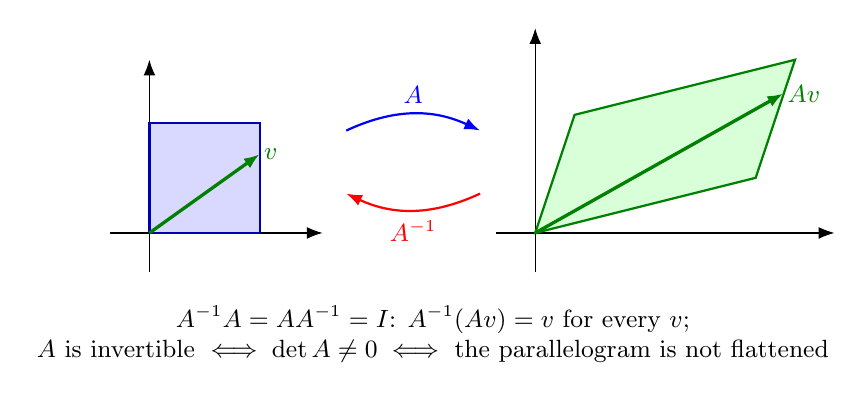
\begin{tikzpicture}[every node/.style={font=\small}, >={Latex[length=2mm]}]
	\draw[->] (-0.5,0) -- (2.2,0);
	\draw[->] (0,-0.5) -- (0,2.2);
	\fill[blue!15] (0,0) rectangle (1.4,1.4);
	\draw[blue!70!black, thick] (0,0) rectangle (1.4,1.4);
	\draw[->, green!50!black, very thick] (0,0) -- (1.4,1.0) node[right, inner sep=1pt, font=\small] {$v$};
	\draw[->, thick, blue] (2.5,1.3) to[bend left=25] node[midway, above] {$A$} (4.2,1.3);
	\draw[->, thick, red] (4.2,0.5) to[bend left=25] node[midway, below] {$A^{-1}$} (2.5,0.5);
	\begin{scope}[xshift=4.9cm]
		\draw[->] (-0.5,0) -- (3.8,0);
		\draw[->] (0,-0.5) -- (0,2.6);
		\fill[green!15] (0,0) -- (2.8,0.7) -- (3.3,2.2) -- (0.5,1.5) -- cycle;
		\draw[green!50!black, thick] (0,0) -- (2.8,0.7) -- (3.3,2.2) -- (0.5,1.5) -- cycle;
		\draw[->, green!50!black, very thick] (0,0) -- (3.15,1.77) node[right, inner sep=1pt, font=\small] {$Av$};
	\end{scope}
	\node[anchor=north, align=center] at (3.6,-0.8) {$A^{-1}A=AA^{-1}=I$: $A^{-1}(Av)=v$ for every $v$;\\ $A$ is invertible $\iff\det A\neq0\iff$ the parallelogram is not flattened};
\end{tikzpicture}
\end{document}
